%%%%%%%%%%%%%%%%%%%%%%%%%%%%%%%%%%%%%%%%%%%%%%%%%%%%%%%%%%%%%%%%%%%%%%%%%%%%%%%%%%%%%%%%%%%%%
%%									Chapitre 4												%
%%%%%%%%%%%%%%%%%%%%%%%%%%%%%%%%%%%%%%%%%%%%%%%%%%%%%%%%%%%%%%%%%%%%%%%%%%%%%%%%%%%%%%%%%%%%%

\chapter{Calcul de Best Matching Unit accéléré avec la topologie}
	\citationChap{
	Il semble que la perfection soit atteinte non quand il n'y a plus rien à ajouter, mais quand il n'y a plus rien à retrancher.
	}{Antoine de Saint-Exupéry}
	\minitoc
	\newpage

%%%%%%%%%%%%%%%%%%%%%%%%%%%%%%%%%%%%%%%%%%%%%%%%%%%%%%%%%%%%%%%%%%%%%%%%%%%%%%%%%%%%%%%%%%%%%



% Début du chapitre			
	\section{Introduction}

	Self-Organizing Maps (SOM) are well-known unsupervised neural networks able to perform vector quantization while mapping an underlying regular neighbourhood structure onto the codebook. They are used in a wide range of applications. As with most properly trained neural networks models, increasing the number of neurons in a SOM leads to better results or new emerging properties. Therefore highly efficient algorithms for learning and evaluation are key to improve the performance of such models. In this paper, we propose a faster alternative to compute the Winner Takes All component of SOM that scales better with a large number of neurons. We present our algorithm to find the so-called best matching unit (BMU) in a SOM, and we theoretically analyze its computational complexity. Statistical results on various synthetic and real-world datasets confirm this analysis and show an even more significant improvement in computing time with a minimal degradation of performance. With our method, we explore a new approach for optimizing SOM that can be combined with other optimization methods commonly used in these models for an even faster computation in both learning and recall phases.

	Self-organizing maps (SOM) are widely used algorithms that feature vector quantization with dimensionality reduction properties. An explanation of how they work can be found in \cite{kohonen2007kohonen}. They are used in numerous fields like image processing, automatic text and language processing, and for visualization, analysis and classification of all kinds of highly dimensional datasets. Many applications examples are depicted in \cite{cottrell:hal-01796059}. However, the amount of computations required by SOMs linearly increases with the number of neurons, the number of elements in the dataset and the dimensionality of the input, in both learning and recall phases. Therefore applying SOMs on datasets with huge numbers of elements and with a high number of neurons to precisely represent the input induces a significant computational cost that may exceed some constraints such as real-time computation or low power consumption.

	With the goal of reducing the required computational time of SOMs in mind, variants of the classical SOM algorithm have been developed. The most well-known SOM modification is the Batch Learning algorithm, as explained in  \cite{cottrell:hal-01796059}. Contrary to the classical online learning, the batch learning averages the modifications over multiple training vectors before updating the neurons weights. Similar efforts have been made in \cite{fiannaca2013simulated} or in \cite{oyana2012new}. However, all those variants are only focusing on reducing the convergence time of the SOM training. To the best of our knowledge, no work has been carried out to reduce the time required for each iteration. This can be partially explained by the highly parallel nature of the computations inside each iterations, in so far as when a fast real world implementation is required, parallel solutions are proposed, like the use of an FPGA substrate with each neuron having its own circuitry, as in \cite{abadi2018scalable} and in \cite{huang2017hardware}. However, parallel solutions should not lead to a lack of effort in optimizing the algorithms, as the majority of SOM training is performed on CPU, and parallel hardware can be costly and difficult to program. Furthermore one can parallelise multiple iterations within an epoch instead of inside the iteration itself, and therefore can benefit from our improvements on parallel hardware.

% -- ICANN Version --
	A SOM training iteration consists of two major parts, a competitive part which searches the Best Matching Unit (or winner neuron), and a cooperative part which updates all the neurons weights proportionally to their distance with the BMU. In the classic SOM, both steps have the same algorithmic complexity (number of neurons multiplied by the dimensionality of the data) and take roughly the same time (depending on implementation details). In this paper we focus on improving the competitive part by reducing the number of neurons evaluated to find the BMU. This optimization also applies to the recall phase.

% -- IJCAI VERSION -- A SOM iteration is composed of two steps during training. The first step consists in finding the Best Matching Unit (or winner neuron), which is done with a comparison between the input vector and the weight vectors of all neurons. The second step consists in modifying the weights of each neuron with regard to its neural distance to the Best Matching Unit. In the classic SOM algorithm, the two steps have the same algorithmic complexity (number of neurons multiplied by the dimensionality of the data) and take roughly the same time (depending on implementation details). In this paper we focus on improving the first step of an iteration by reducing the number of comparisons required to find the Best Matching Unit (BMU). This optimization also applies to the recall phase that reduces to the first step for each new input pattern.

	After a brief description of the standard SOM model in section \ref{seq:som}, section \ref{seq:algorithm} defines the proposed method to speed up the computation of BMU, before analyzing its computational complexity. The experimental setup is described in section \ref{seq:exp_setup}, 
%including various datasets and the definition of the associated performance measures. 
	and the corresponding results are discussed in section \ref{seq:results}.


	\section{Observations topologiques}
	\newpage
	\section{Algorithme séquentiel}
	\subsection{Algorithme}

	We present here our new algorithm for searching the Best Matching Unit (BMU) in the SOM. It is traditionally determined by means of an exhaustive search by comparing all the distances between the input vector and the neurons weights. This method, while able to always find the correct minimum of the map, is computationally inefficient. The dimensionality reduction property of the SOM means that close neurons in the SOM topology represent close vectors in the input space. Therefore when an input vector is presented to the SOM, a pseudo-continuous gradient appears in the SOM when considering the distances between the neuron weights and the input vector whose minimum is located at the BMU. 
	%Using some kind of discretized gradient descent approach, we expect that this distance will progressively reduce until the Best Matching Unit is reached, with the minimal distance in the map. 

	\begin{algorithm}[tb]
	\caption{Particle}
	\label{alg:particle}
	\textbf{Input}: $pos$ : current position\\
	\textbf{Parameters}: $values$: global table of distances, $eval$: global history of evaluations \\
	\textbf{Output}: $bmu$ : best matching unit's index
	\begin{algorithmic}[1] %[1] enables line numbers
	\IF {$eval(pos)$ is True}
	\STATE \textbf{return} $pos$
	\ENDIF
	\STATE $eval[pos] \xleftarrow{}$ True
	\STATE Let $new\_pos$ take the index of the closest not evaluated neighbour to the input vector (ignoring neighbours $p$ such that $eval(p)=$True)
	\IF {$values[new\_pos] \leq values[pos]$}
	\STATE \textbf{return} Particle($new\_pos$)
	\ENDIF
	\STATE \textbf{return} The index of the smallest value between $pos$ and the returned indexes by execution of Particle() on all direct neighbours of $pos$.
	\end{algorithmic}
	\end{algorithm}

	In our algorithm we use this progressive reduction of distances to perform a discretized gradient descent to find the Best Matching Unit. The pseudo-code is shown in Algorithm \ref{alg:particle}, and illustrated in figure \ref{fig:first_particle} (left). The algorithm starts at an arbitrarily selected position in the map. For this example let us consider that it starts at coordinates $(0,0)$ (top left corner). This neuron has two neighbours, one to the east (1,0) and one to the south (0,1). We evaluate the distances to the input vector of these three neurons to find the next step in the gradient descent. If the smallest distance is found where we are currently positioned, then we consider this is a local minimum. On the contrary if one of the neighbouring neurons gives the smallest distance, then the gradient descent goes in the direction of this particular neuron, that becomes the next selected position from which we repeat this process until we find a local minimum. In our example the smallest distance is measured for the eastern neuron in (1,0). Thus the search process moves one step to the east, and this neuron has three neighbours, one to the south (1,1), one to the east (2,0) and one to the west that we come from (and thus we ignore it). We compare the three distances again, and move towards the lowest distance (south).

	This process iterates until it reaches a local minimum at position (6,5), where all neighbouring neurons have a higher distance to the input vector than the selected neuron. In order to ensure that the local minimum that has been found is the best one in the local neighbourhood, we then perform a search of the local space by continuing the gradient descent from all directly neighbouring neurons that are still unexplored. If this search finds a better local minimum, then this local minimum is considered as the BMU. This part of the algorithm aims at circumventing problems that may arise from the topology. In a grid topology for instance, we can only look at orthogonal axes. But sometimes, the gradient is oriented towards a diagonal direction, and by extending the search from a local minimum, we are able to still follow this gradient towards a potential BMU.

	\begin{figure}[!t]
    	\centering
    	\includesvg[scale=1.2]{first_particle}\ \ \ \ \ \ \ 
    	\includesvg[scale=1.2]{all_particles}
    	\caption{Left: Example of the execution of one particle. Each cell represents one neuron. The arrow in each cell points towards the best neighbour (where a lower distance can be found). A star represents a local minimum. The green colored cells are the neurons who have been explored during the search, and the blue cells are the neurons whose distance to the input has been computed but that have not been explored by the algorithm. After having found a local minimum, new particles are created (in red) and continue the gradient descent by exploring the local neighbourhood. The cell in Yellow is the BMU, and the global minimum of the map. Right: Execution of the four particles.}
    	\label{fig:first_particle}
	\end{figure}

	Another problem that can arise with the particle algorithm is edge effects. When mapping high dimensional data onto a 2D map, the map sometimes become twisted  no gradient between the top left neuron and the bottom right neuron. Imagine a net that is thrown onto a ball and nearly completely enveloping it: the shortest path between one corner of the net and the opposite corner of the net does not follow the mesh of the net. If in the learning phase, the particle ends up in the wrong corner of the SOM, it will find a terrible BMU and the following weight update will locally break the neighbourhood continuity, and create a negative feedback loop that will remove all dimensionality reduction properties from the SOM. Thankfully there is an easy way to avoid this, by simply starting 4 particles, one in each corner of the SOM, and selecting the smallest BMU found. This technique preserves the continuity of the SOM and makes the Fast-BMU algorithm more robust to local discontinuities in the gradient, especially at the beginning of the training process, when the map is not yet well unfolded. In the case where there is no clear gradient present in the SOM (typically when the SOM is randomly initialized before training), this algorithm will fail to find the correct BMU. However it is not a problem at the start of training as the neighborhood function will create a gradient by unfolding the SOM regardless of which neuron is initially selected. The result of a full Fast-BMU execution is shown in figure \ref{fig:first_particle} (right).

	\subsection{Analyse de la complexité}

	Le temps d'exécution d'une recherche de BMU dans la SOM classique dépend de deux facteurs : le nombre de neurones multiplié par la durée d'une comparaison entre le vecteur d'entrée et les poids d'un neurone. L'idée de Fast-BMU étant de réduire le nombre de ces comparaisons, la durée d'une comparaison ne sera pas prise en compte dans cette analyse. C'est normalement une valeur constante qui ne dépend que de la dimensionalité des données. Le nombre de comparaisons pour Fast-BMU est quand à lui dépendant de la taille de la carte, c'est à dire hauteur et largeur, et de la topologie, c'est à dire du nombre de voisins par neurone. 

	Étant donné que notre algorithme ne fonctionne que si 

As our algorithm relies on the dimensionality reduction property of the SOM, we will hypothesise that there is always some kind of continuity in the neural map in our analysis, because if not, our algorithm would not work anyways.

	In order to estimate the complexity of our algorithm, we have to estimate the number of steps that each of the four particles takes before finding a potential Best Matching Unit (BMU). We assume that: 1) all particles follow paths that do not significantly differ from shortest XY paths until their destination (thus minimizing the number of steps), and 2) they do not stop early in some local minimum (thus maximizing the number of steps). We will call this kind of  best-worst-case complexity: \textit{Expected Complexity}.

	Let us consider that the BMU is located at position $x, y$ of the SOM : 
	\begin{itemize}
    	\item The top left particle with coordinates $(0,0)$ needs $x$ steps in the width dimension, and $y$ steps in the height dimension in order to get to the BMU.
    	\item Similarly, the top right particle with coordinates $(w,0)$ will take $w-x$ steps for the width and $y$ steps for the height.
    	\item For the bottom left $(0,h)$, it will be $x$ and $h-y$ steps.
    	\item For the bottom right $(w,h)$, it will be $w-x$ and $h-y$ steps.
	\end{itemize}

	To get the total number of steps for one execution, we sum the steps from all particles together as shown in equation \ref{eq:nbsteps}:
	\begin{align}\label{eq:nbsteps}
    	\text{NbSteps} = (x + y) + (w - x + y) + (x + h - y) + (w - x + h - y) 
	\end{align}

	The $x$ and $y$ cancel out, and the resulting number of steps only depends on the width and the height of the map. The total number of steps taken by our algorithm is consequently equal to $(2w + 2h)$. 
	% Each particle therefore has an average number of steps equal to $\frac{(w+h)}{2}$ in our case. 
	We can therefore derive equation \ref{eq:complexity}, which defines the expected complexity of our algorithm.

	\begin{align}\label{eq:complexity}
    	{\cal EC}(w, h) = 2 \times (w + h) \times NbrEvalPerStep
	\end{align}

	with $w, h$ the width and height of the SOM respectively and $NbrEvalPerStep$ the number of new distances to compute on each step of a particle. Its value depends on the topology. It is at most 3 with a grid (4 neighbours minus the neuron from the previous step) and also 3 with a hexagonal topology (6 neighbours minus the neuron from the previous step and 2 neurons that were neighbours of the previous neuron and consequently have already been evaluated). 

	From an analytical point of view, we can estimate that our Fast-BMU algorithm (${\cal EC}(w,h)=6(w+h)$ in the worst case in a standard grid configuration) is significantly faster than the current exhaustive search algorithm (O$(w,h) = wh$) when the number of neurons in the map is substantial. For instance, it is twice as fast with 24 by 24 SOMs, and 10 times faster with 120 by 120 SOMs. An experimental evaluation of the speed difference is reported in section \ref{seq:results}.

	\subsection{Protocole expérimental}

	To evaluate the robustness of our algorithm with various kinds of data, we have selected 6 datasets aimed at being representative of the kind of data SOMs are usually trained on. For the 2D case, we have generated data with different properties (uniform distribution and a highly non-convex shape), for 3D data we use a uniformly distributed cube shape and the pixel color values of an image. For the high dimensional case, we consider an image compression application \cite{amerijckx2003image} with 10 by 10 sub-images as training vectors (100 pixels with 3 colors each, resulting in 300 dimensions), and the Free Spoken Digits Dataset \cite{zohar_jackson_2018_1342401} which uses soundwaves that we have reduced to 1000 dimensions.

	Our algorithm is mostly designed for a 2 dimensional SOM, although adaptations to higher dimensions can be easily defined by just adapting the neighbourhood and the number of initial particles, even leading to possibly greater gains in computational cost. We tested it with a grid and a hexagonal shaped 2D topology, which are the most commonly used in SOM applications. 
%Other topologies could work, but it is necessary to keep a strong continuous dimensionality reduction property through the topology (close neighbours should have close weights).

	In order to evaluate the differences between all tested models, we used three metrics. The first one is the standard \textit{Mean Squared Quantization Error} (MSQE) which estimates the Vector Quantization quality of the tested algorithm. The \textit{Mean Squared Distance to Neurons} (MSDtN) which computes the average squared codeword distance between neurons and all of their direct neighbours. The lower this value is, the more closely related neighbouring neurons are, and the better the dimensional reduction property is. Numerous metrics exist in the SOM literature to estimate the topographical mapping of the SOM, but MSDtN has the advantage of being easy to compute, without parameters and only dependent on the neurons weights. For all metrics, lower is better. 

	\begin{equation}
    	\text{MSQE} = \frac{1}{V} \sum_{i=1}^{V} ||v_i - w_{\text{bmu}(i)}||^2
	\end{equation}

	\begin{equation}
    	\text{MSDtN} = \frac{1}{N} \sum_{i=1}^{N} \sum_{j=1}^{N} 
    	\begin{cases}
        	||w_i - w_j||^2,  & \text{if dist}(i, j) = 1\\
        	0,              & \text{otherwise}
    	\end{cases}
	\end{equation}

	With $V$ the number of vectors in the dataset, $v_i$ the weights of the $i^{th}$ vector of the dataset, and bmu($i$) is the index of the neuron which is the best matching unit for the $i^{th}$ vector of the dataset. Similarly $N$ is the number of neurons and $w_i$ the weights of the $i^{th}$ neuron, while dist($i, j$) is the number of links in the shortest path between neurons $i$ and $j$ in the neural map.

	\subsection{Résultats}
	\subsubsection{Performances}

	In this section, we explore the differences in quality of learning and recall between the standard version and our fast version for the computation of the BMU in a SOM. We also look at the practical differences in the amount of computations required for the two versions and we compare it with the previously presented complexity analysis.
	
	Quality tests were performed on a $32\times32$ SOM (1024 neurons). For each combination of dataset and model (choice of topology and BMU algorithm), we ran 50 executions with different random seeds which affect the datasets that are generated, the initialization of the neuron weights (who are all randomly initialised with no pre-existing gradient) and the order in which the training vectors are presented. Results are shown in table \ref{tab:results}.

	The algorithm column of the table shows the combination of BMU finding algorithm and topology that was used for training. The MSDtN (see section \ref{seq:exp_setup}) is calculated on the trained neurons weights. The MSQE\_S (Standard) is the quantization error in the recall phase (after learning) when using the standard BMU algorithm. Comparing the different MSQE\_S values for a standard version and a fast version gives an indication of the influence of the Fast-BMU algorithm on training quality only, as it always selects the real BMU in the recall phase. The MSQE\_F (Fast) metric measures the vector quantization error with the BMU selection done by the Fast-BMU algorithm. If the training was performed on the standard SOM, it gives an indication of the influence of the Fast-BMU algorithm on recall accuracy only; if it was trained on a Fast version, it represents the MSQE result of a SOM that only uses the Fast-BMU algorithm. The mismatch column gives the proportion of BMU that are selected differently by the two algorithms.

	\begin{tableth}
	\label{tab:recap:param}
	\caption[Résultats de FastBMU sur différentes données]{Results with a 32x32 neurons SOM, averaged over 50 executions. The Algorithm column specifies with which algorithm and topology the SOM was trained, FastG and FastH stand respectively for Fast Grid and Fast Hexagonal. MSQE\_S is the MSQE calculated with the standard (exhaustive) BMU algorithm whereas MSQE\_F uses the Fast-BMU version. Differences of MSQE\_S between different algorithms reflect the quality of the training phase. The mismatch is the proportion of BMU that are differently selected by the two algorithms.}
	\begin{tabular}{|c|l|r|r|r|r|}
	\hline
	Données & Algorithme & MSDtN & MSQE\_S & MSQE\_F & Mismatch\\
	\hline
	Carré 	& Grille  & \nbr{1.94e-4} & \nbr{2.22e-4} & \nbr{2.22e-4} & 0\%\\
    (2D)   	& Fast-Grille & \bst{1.93e-4} & \nbr{2.23e-4} & \nbr{2.23e-4} & 0\%\\
        	& Hexagonal	& \nbr{2.39e-4} & \bst{2.12e-4} & \bst{2.12e-4} & 0\%\\
        	& Fast-Hexa	& \nbr{2.38e-4} & \nbr{2.15e-4} & \nbr{2.15e-4} & 0\%\\
	\hline
	Forme   & Grille  & \bst{1.38e-4} & \nbr{1.40e-4} & \nbr{1.40e-4} & $\approx$0\%\\
    (2D)    & Fast-Grille & \bst{1.38e-4} & \nbr{1.40e-4} & \nbr{1.40e-4} & $\approx$0\%\\
        	& Hexagonal   & \nbr{1.65e-4} & \bst{1.31e-4} & \bst{1.31e-4} & $\approx$0\%\\
        	& Fast-Hex & \nbr{1.65e-4} & \bst{1.31e-4} & \bst{1.31e-4} & $\approx$0\%\\
	\hline
	Cube   	& Grille  & \bst{4.48e-4} & \nbr{2.21e-3} & \nbr{2.50e-3} & 4.8\%\\
    (3D)   	& Fast-Grille & \nbr{4.61e-4} & \nbr{2.25e-3} & \nbr{3.21e-3} & 9.8\%\\
        	& Hexagonal   & \nbr{5.29e-4} & \bst{2.09e-3} & \bst{2.34e-3} & \bf{3.1\%}\\
        	& Fast-Hex & \nbr{5.38e-4} & \nbr{2.11e-3} & \nbr{2.79e-3} & 7.6\%\\
	\hline
	Couleurs& Grille  & \bst{1.15e-4} & \nbr{8.64e-5} & \nbr{8.80e-5} & 4.4\%\\
    (3D)    & Fast-Grille & \nbr{1.19e-4} & \nbr{8.91e-5} & \nbr{9.08e-5} & 5.4\%\\
        	& Hexagonal   & \nbr{1.33e-4} & \nbr{8.29e-5} & \nbr{8.30e-5} & \bf{0.4\%}\\
       		& Fast-Hex & \nbr{1.35e-4} & \bst{8.26e-5} & \bst{8.29e-5} & 0.7\%\\
	\hline
	Sons    & Grille  & \nbr{2.02e-4} & \nbr{1.42e-2} & \nbr{1.49e-2} & 31.3\%\\
    (2D)   	& Fast-Grille & \bst{1.93e-4} & \nbr{1.44e-2} & \nbr{1.51e-2} & 32.2\%\\
        	& Hexagonal   & \nbr{2.29e-4} & \bst{1.41e-2} & \bst{1.45e-2} & 19.8\%\\
        	& Fast-Hex & \nbr{2.25e-4} & \nbr{1.42e-2} & \bst{1.45e-2} & \bf{13.3\%}\\
	\hline
	Image  	& Grille  & \bst{1.64e-4} & \nbr{1.80e-3} & \nbr{1.83e-3} & 4.2\%\\
    (2D)    & Fast-Grille & \nbr{1.65e-4} & \nbr{1.82e-3} & \nbr{1.85e-3} & 4.4\%\\
        	& Hexagonal   & \nbr{1.97e-4} & \bst{1.75e-3} & \nbr{1.77e-3} & \bf{1.2\%}\\
        	& Fast-Hex & \nbr{1.99e-4} & \bst{1.75e-3} & \bst{1.76e-3} & \bf{1.2\%}\\
	\hline
	\end{tabular}	
	\end{tableth}

	We first observe that the distance between neurons after learning (MSDtN) is lower with the grid topology than with the hexagonal one, but this difference could be attributed to the different number of neighbours between the two topologies and therefore should only be used to compare the standard and Fast-BMU algorithms, and not topologies. We also remark that the Fast algorithm does not make any significant mismatch on the Square and Shape datasets, and therefore MSQE\_S and MSQE\_F have similar recall results on these datasets.

	The mismatch percentages vary greatly between the datasets. From 0 to 6\% for the Images and Colors Datasets, 3 to 10\% for the Cube and 13 to 33\% for the Spoken Digits dataset. Such differences could be explained by the distribution of the data in the datasets, as Images and Colors feature data that are closely related together. In pictures for instance, there are usually a few dominant colors with a lot of color gradients that make the continuities in the distribution easier to learn for the SOM, thus improving the performance of our Fast-BMU algorithm. The Spoken Digits dataset on the other hand has high mismatch values, which seems to indicate that a strong continuity in the neurons weights is not present after learning the SOM. The hexagonal topology also performs better with the Fast-BMU algorithm than the grid topology as mismatches are significantly lower with it. Finally the dimensionality of the dataset does not seem to play a key role here, as the Image dataset (300 dimensions) has lower mismatches than the Cube dataset (3 dimensions).

	For the vector quantization part, the hexagonal topology leads again to the lowest error values. What is more surprising is that the Fast-BMU version has quantization results that are very similar to the standard version. Even with high mismatches (30\% with Digits using a grid-based SOM) the MSQE is only around 5\% higher, and even less when only training is compared. The only significantly higher MSQE values with Fast-BMU is with the Cube dataset where the algorithm selects quite bad BMU choices in the recall phase while being able to correctly train the SOM. In most cases, a difference in the topology of the SOM has more impact on the resulting MSQE than the use of the Fast-BMU algorithm. 

	\subsubsection{Gain computationnels}

	\begin{figureth}
    	\centering
    	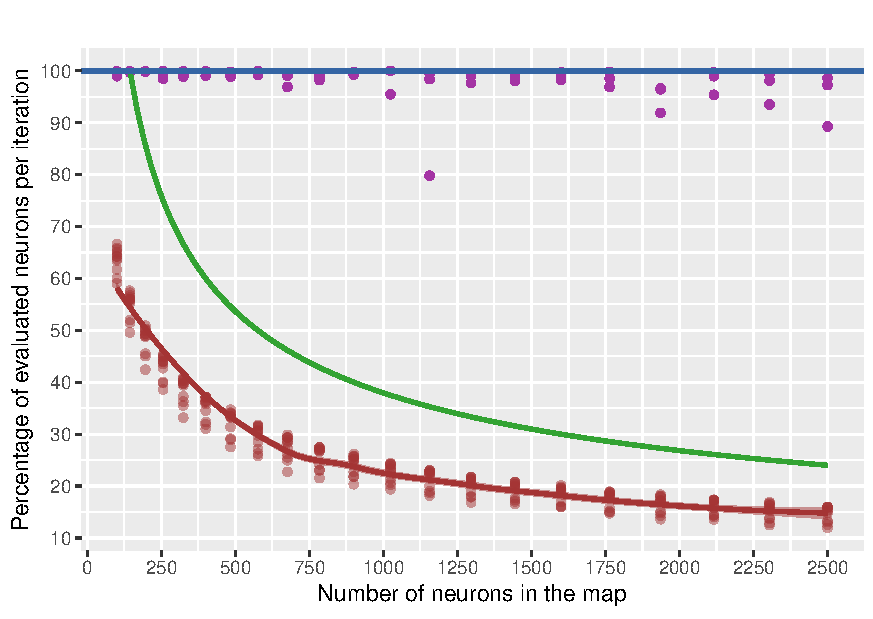
\includegraphics[width=1\textwidth]{performance_diff.pdf}
	%    \includesvg[inkscapelatex=false, width=0.8\textwidth]{performance_diff.pdf}
    	\caption{Evaluation of performance gains with the number of neurons. All results were calculated on square maps. The blue line is the standard SOM, in green is the analytical value and in red the measured value. Additionally, the purple dots are the percentage of correct BMU in an execution on the Image dataset.}
    	\label{fig:performance_diff}
	\end{figureth}


	To evaluate the computational gains that are induced by the use of the Fast-BMU algorithm independently from implementation techniques, we compared the percentage of neurons that must be evaluated in order to find the BMU. The results are shown in figure \ref{fig:performance_diff}. The standard SOM is evaluating all neurons by definition, so the percentage is always 100\%. The complexity curve for Fast-BMU plots the function defined in section \ref{seq:complex_analysis}. To obtain the Fast-measured curve, we ran tests with $n\times n$ SOM, where $n$ is every even number between 10 and 50 (21 tests in total). Each test featured all datasets and all topologies (so 12 executions per test). 

	With these results, we can observe significant improvements in the required computational time. Our algorithm is twice as fast with $(16\times16)$ SOMs, four times faster with 1000 neurons ($32\times32$). The ($50\times50$) SOM evaluates approximately 375 neurons per iteration, which is similar to the 400 neurons a standard ($20\times20$) SOM has to evaluate. We can also observe that the complexity curve follows a similar shape to the measured curve, while overestimating the required number of evaluated neurons by approximately 75\%.	

	\newpage
	\section{Algorithme parallèle}
	\section{Conclusion}

	We have presented a novel method to find the Best Matching Unit in Self-Organizing Maps by taking advantage of their ability to preserve their underlying topology within the codebook. Our algorithm is significantly faster to compute while performing barely worse than the standard approach in vector quantization. %The difference in vector quantization is not a significant problem, since it can be compensated by using slightly larger neural maps that are faster to compute with our method. 

	This result makes SOM with a high number of neurons a more viable solution for many applications. We expect future improvements of this algorithm, or new approaches to further reduce the computational cost of SOM by modifying the BMU searching algorithm. We also study how the Fast-BMU approach can reduce the bandwidth demands in a fully parallel implementation on a manycore substrate, where all neurons are simultaneously evaluated but the BMU selection uses the simple unicast propagation of particles instead of full broadcast-reduce schemes. Finally it must be pointed out that the computational gains offered by our Fast-BMU algorithm specifically rely on preservation of neighbourhood relations when mapping the input space onto the neural map. This property is not present when using more conventional VQ models such as k-means, so that the use of SOM could be extended to more applications where their specific mapping properties would not be useful for the application itself, but would induce potential computational gains out of reach for other models.
		
\bibliographystyle{francaissc}
\bibliography{Chapitre4/Biblio}